\documentclass[journal]{IEEEtran}

\usepackage{amsmath,amssymb}
\usepackage{booktabs}
\usepackage{multirow}
\usepackage{array}
\usepackage{tabularx}
\usepackage{graphicx}
\usepackage{adjustbox}
\usepackage[table]{xcolor}
\usepackage{cite}
\usepackage{url}
\usepackage{balance}

\newcommand{\method}{VK-RMD}
\newcommand{\mpjpe}{MPJPE}
\newcommand{\pampjpe}{PA-MPJPE}
\newcommand{\gain}[1]{\textcolor{green!45!black}{#1}}
\newcommand{\loss}[1]{\textcolor{red!70!black}{#1}}
\newcommand{\neutral}[1]{\textcolor{gray!70!black}{#1}}

\begin{document}

\title{\method: Availability-Conditioned Structural Evidence Learning for Reduced-Exposure Multimodal Human Perception}

\author{Author Name,
        \IEEEmembership{Member, IEEE}
\thanks{The author is with the School of Computer Science and Technology, Dalian University of Technology, Dalian, China. E-mail: author@example.com.}
}

\markboth{IEEE Internet of Things Journal,~Vol.~XX, No.~XX, 2026}
{Author \MakeLowercase{\textit{et al.}}: \method{} for Reduced-Exposure Multimodal Human Perception}

\maketitle

\begin{abstract}
Multimodal human perception is often built around raw RGB or fixed sensor configurations, yet downstream HPE and HAR systems may need to operate without raw visual streams and under changing sensor availability. This paper presents \method, an availability-conditioned structural-evidence framework for missing-modality multimodal human perception. Visual keypoints (VK) are used as a compact structural interface rather than as a formal privacy guarantee: if visual input is used upstream, the downstream perception model receives only VK and non-RGB sensors. The framework maps VK, depth, LiDAR, mmWave, and WiFi-CSI into task-supervised human-state tokens, trains a full-observation reference model and randomly subset-conditioned students, and combines local chunk evidence with a global fused-token readout using learned contribution proxies. Direct X-Fi table comparisons show that the full HPE setting improves from 83.7 mm to 50.2 mm MPJPE and the full HAR setting improves from 72.2\% to 96.6\% accuracy. The complete subset tables report both gains and failures for individual sensing conditions. A subject-identification probe shows that VK reduces predictability compared with defaced RGB but remains above chance; therefore, the privacy claim is limited to reduced visual exposure and raw-RGB-free downstream inference.
\end{abstract}

\begin{IEEEkeywords}
Internet of Things, multimodal sensing, human pose estimation, human activity recognition, missing modality, visual keypoints, reliability-aware fusion, reduced visual exposure.
\end{IEEEkeywords}

\section{Introduction}
\IEEEPARstart{M}{ultimodal} human perception is becoming an important function in sensor-rich Internet-of-Things (IoT) environments, including intelligent buildings, assisted living, contactless interaction, and human-centered monitoring. Human pose estimation (HPE) provides fine-grained body geometry, whereas human activity recognition (HAR) provides action-level semantics. A useful IoT perception system should therefore support both structural and semantic understanding. In practice, however, the sensing environment is rarely ideal. Cameras may be restricted by policy, depth cameras may be occluded, LiDAR and mmWave point clouds may be sparse, and radio-frequency signals may be environment dependent. Robust perception must therefore handle reduced visual exposure and missing sensor modalities at the same time.

Raw RGB frames are informative, but they expose face, clothing, body appearance, and scene background. For long-term deployment, it is therefore useful to decouple the downstream perception model from raw RGB streams. This does not require claiming that the structural representation itself is anonymous. Instead, the key question is whether a compact structural interface can replace raw RGB inside the deployable perception model. Visual keypoints (VKs) provide such an interface: they preserve joint topology and motion-relevant geometry while suppressing most texture, color, face, and background appearance. VK can be produced by an upstream visual module, a defaced or edge-side process, or other keypoint-estimation sources; the downstream HPE/HAR model in this work does not consume raw RGB.

We identify two coupled bottlenecks behind this problem. The first is the structural-interface gap: once raw RGB is removed from the downstream model, heterogeneous sensors still need a compact body-structure interface that can organize pose and action evidence. The second is subset instability: the relative contribution of VK, depth, LiDAR, mmWave, and WiFi-CSI changes when the available sensor set changes. A model that performs well under complete inputs can therefore fail when one or more sensors are absent.

We propose \method{} as an availability-conditioned structural-evidence learning algorithm built around an RGB-optional structural interface. VK tokenization addresses the structural-interface gap by representing body geometry as joint-aware tokens and mapping heterogeneous sensors into a common task-supervised token dimension. Subset-conditioned learning addresses availability instability by training over randomly sampled modality subsets. The readout preserves modality chunks for local task evidence and also forms a global fused-token prediction; learned uncertainty is used only as a contribution proxy. Auxiliary teacher supervision stabilizes the full-observation-to-subset transition, but is not presented as a new distillation category.

This work is positioned as an engineering-oriented IoT sensing study with an explicit algorithmic structure. The contribution is not the isolated invention of keypoints, attention, or modality sampling. Instead, we formulate reduced-exposure human sensing as a two-bottleneck problem and instantiate a two-mechanism solution. The experimental design includes all 31 HPE modality combinations, all 15 HAR modality combinations, non-visual students, cross-scene and cross-subject splits, fair internal baselines, and reliability diagnostics.

The main contributions are summarized as follows.
\begin{itemize}
    \item We formulate RGB-optional multimodal human perception as a missing-modality learning problem with two bottlenecks: structural-interface learning and subset instability.
    \item We develop an availability-conditioned structural-evidence formulation that combines VK-based task-supervised tokenization, random subset training, and chunk-preserving/global readout for raw-RGB-free HPE and HAR.
    \item We establish the mechanism boundaries with matched VK-input baselines, loss-profile ablations, all-combination evaluation, cross-protocol tests, contribution-proxy diagnostics, and a subject-ID probe that bounds the reduced-exposure claim.
\end{itemize}

\section{Related Work}

\subsection{IoT Human Sensing and Reduced Visual Exposure}
IoT human sensing uses distributed sensors to infer human state, motion, and activities. Vision-based approaches provide rich information but raise exposure concerns in long-term deployment. Non-visual sensing with depth, RF, radar, and point clouds can reduce direct visual exposure, but usually sacrifices signal richness or becomes sensitive to environment layout. Skeletons and visual keypoints are widely used as compact body-structure representations in pose estimation and action recognition \cite{openpose,stgcn}. In this paper, VK is not treated as a secure representation; it is treated as an RGB-optional structural interface that enables the downstream model to avoid raw RGB input.

\subsection{Multimodal HPE and HAR}
HPE estimates joint-level body structure, whereas HAR predicts action categories. Multimodal datasets such as MMFi \cite{mmfi} make it possible to evaluate visual, depth, LiDAR, mmWave, and WiFi-CSI streams under the same action and pose labels. X-Fi \cite{xfi} is a particularly relevant baseline because it studies flexible multimodal human sensing. Our work uses X-Fi/VK as a reproduced or official baseline and focuses on the missing-modality robustness that remains difficult when arbitrary modality subsets must be supported.

\subsection{Missing-Modality Learning}
Missing-modality learning has been studied through modality dropout, reconstruction, hallucination, mixture-of-experts, and knowledge transfer \cite{missing}. Many methods use random modality removal as regularization. In contrast, our setting treats each sampled subset as a valid deployment condition and evaluates all valid combinations. This distinction matters: a model is not considered robust merely because it tolerates one manually selected missing case.

\subsection{Reliability-Aware Fusion and Auxiliary Teacher Signals}
Adaptive multimodal fusion can outperform fixed concatenation or uniform averaging when sensor quality varies. Uncertainty-aware and attention-based fusion strategies have been used to weight heterogeneous information \cite{kendall2017,transformer}. We use reliability-aware weights as task-level learned contribution proxies. Knowledge distillation \cite{hinton2015,fitnets} and privileged information \cite{vapnik2009} motivate stronger training signals for restricted students. In this paper, teacher supervision is auxiliary; the main contribution is the subset-conditioned body-token learning formulation.

\subsection{Positioning Against Closest Paradigms}
The closest prior directions each explain part of the design, but none directly matches the proposed setting. X-Fi studies flexible multimodal human sensing and provides an important baseline, but its central formulation remains modality-invariant sensing rather than RGB-optional structural-interface learning. General missing-modality methods often treat modality removal as a robustness or reconstruction problem, whereas \method{} treats every sampled subset as a deployable sensing configuration and evaluates the full modality-availability space. Knowledge distillation transfers outputs or intermediate hints from a teacher, while our use of teacher supervision is full-modality-to-subset transfer: the student is not merely smaller, but input-restricted. Skeleton-based methods such as ST-GCN use keypoints for recognition, whereas \method{} uses VK as a structural interface through which heterogeneous sensors are organized in a task-supervised body-latent token space. These differences matter because the target problem jointly requires raw-RGB-free downstream inference, heterogeneous sensor organization, and arbitrary sensor availability.

\section{VK-RMD Framework}

\subsection{Problem Definition}
Let $\mathcal{M}_{p}=\{\mathrm{VK},D,L,R,W\}$ denote the HPE modality set, where $D$, $L$, $R$, and $W$ denote depth, LiDAR, mmWave, and WiFi-CSI. Let $\mathcal{M}_{a}=\{\mathrm{VK},D,L,R\}$ denote the HAR modality set. For each sample, only a non-empty subset $\mathcal{S}\subseteq \mathcal{M}$ may be available. The student receives $\mathbf{x}_{\mathcal{S}}=\{\mathbf{x}_{m}:m\in\mathcal{S}\}$ and predicts either a 3D pose $\hat{\mathbf{Y}}$ or an action probability vector $\hat{\mathbf{p}}$.

For HPE, the target is a 17-joint 3D pose. The primary metric is \mpjpe{} in millimeters; lower values are better. For HAR, the target is one of 27 actions; accuracy and macro-F1 are used, and higher values are better. The training objective is to make $f_{\theta}(\mathbf{x}_{\mathcal{S}},\mathcal{S})$ reliable for all possible modality subsets, not only for the full set.

\subsection{Formal View of VK-Mediated Body-Latent Tokenization}
VK is represented as a 17-joint body graph rather than a generic coordinate array. Let $\mathbf{x}_{v}\in\mathbb{R}^{17\times 2}$ denote the VK input. We view it as $G_v=(V,E,X)$, where $V$ contains semantic joint identities, $E$ is the skeleton topology, and $X$ is the coordinate observation. The VK encoder normalizes the coordinates, adds coordinate, position, and joint-identity embeddings, and propagates information over the bone graph:
\begin{equation}
    \mathbf{J}_{v}=\phi_c(\tilde{\mathbf{x}}_v)+\phi_p(2\tilde{\mathbf{x}}_v-1)+\mathbf{e}_{joint},
\end{equation}
\begin{equation}
    \mathbf{J}_{v}^{(k+1)}=\mathrm{BoneGraphMixer}(\mathbf{J}_{v}^{(k)}, A_{bone}),
\end{equation}
\begin{equation}
    \mathbf{Z}_{v}=P_v(\mathbf{J}_v)\in\mathbb{R}^{K\times D}.
\end{equation}
For each non-VK modality $m$, a modality-specific backbone and trainable projector produce body-latent tokens:
\begin{equation}
    \mathbf{Z}_{m}=P_m(E_m(\mathbf{x}_m))\in\mathbb{R}^{K\times D}.
\end{equation}
The raw spaces are therefore not aligned directly. A WiFi-CSI tensor, a LiDAR point cloud, a radar point set, and VK coordinates are first mapped into a shared body-latent token dimension. We use the term body-latent tokenization rather than strict semantic alignment: the correspondence is induced by sample-level synchronization, common HPE/HAR supervision, modality embeddings, and the VK skeleton topology, but it is not a guaranteed geometric registration.

For an available subset $\mathcal{S}$, modality embeddings are added and concatenated:
\begin{equation}
    \mathbf{U}_{\mathcal{S}}=\mathrm{Concat}_{m\in\mathcal{S}}(\mathbf{Z}_{m}+\mathbf{e}_{m}),
\end{equation}
\begin{equation}
    \mathbf{T}_{\mathcal{S}}=\mathrm{TransformerEncoder}(\mathbf{U}_{\mathcal{S}}).
\end{equation}
The encoded tokens are split into modality chunks $\{\mathbf{T}_m\}_{m\in\mathcal{S}}$. Each chunk produces a modality-wise pose or action expert and a log-variance score $s_m$. The default reliability-guided fusion uses
\begin{equation}
    \alpha_m=\frac{\exp(-s_m/\tau)}{\sum_{j\in\mathcal{S}}\exp(-s_j/\tau)}.
\end{equation}
For HPE, the modality-wise pose experts and residual fused token head are combined as
\begin{equation}
    \hat{\mathbf{Y}}=0.5\sum_{m\in\mathcal{S}}\alpha_m\hat{\mathbf{Y}}_m+
    0.5H_{res}\left(\sum_{m\in\mathcal{S}}\alpha_m\mathrm{Pool}(\mathbf{T}_m)\right).
\end{equation}
For HAR, the same mechanism is applied to logits:
\begin{equation}
    \hat{\mathbf{c}}=0.5\sum_{m\in\mathcal{S}}\alpha_m\hat{\mathbf{c}}_m+
    0.5H_{res}\left(\sum_{m\in\mathcal{S}}\alpha_m\mathrm{Pool}(\mathbf{T}_m)\right).
\end{equation}
The weights $\alpha_m$ are learned contribution proxies. They should not be interpreted as calibrated physical reliability values.

\subsection{Two Challenges: Structural Interface and Subset Instability}
The proposed framework is organized around two challenges. The structural-interface challenge arises because raw RGB provides strong body and context information, but the downstream model is designed to operate without raw RGB. Non-RGB sensors are more suitable for reduced-exposure deployment, yet they do not naturally provide the same explicit body structure. The subset-instability problem arises because the available modality set changes across deployment conditions. A fixed fusion rule cannot assume that a modality has the same contribution in every subset.

\method{} addresses the structural-interface challenge through VK-anchored body-tokenization and addresses subset instability through reliability-guided subset learning. This problem-mechanism mapping is the main algorithmic logic of the paper.

\subsection{VK-Anchored Body-Tokenization}
Fig.~\ref{fig:framework} shows the overall framework. Raw visual data, if used, is isolated in the upstream VK extraction stage; the downstream model receives VK rather than raw RGB. VK is then encoded as joint-level body geometry. Other modalities use their own encoders because their raw forms are heterogeneous: depth images, point clouds, radar points, and WiFi-CSI sequences cannot be aligned directly in raw space. For modality $m$, the feature is encoded as
\begin{equation}
    \mathbf{z}_{m}=P_m(E_m(\mathbf{x}_{m}))+\mathbf{e}_{m},
\end{equation}
where $E_m$ is a modality-specific encoder, $P_m$ is a projection layer into the shared body-token dimension, and $\mathbf{e}_{m}$ is a modality embedding. Alignment is therefore performed in the body-token space and is driven by common HPE/HAR supervision.

\begin{figure}[t]
    \centering
    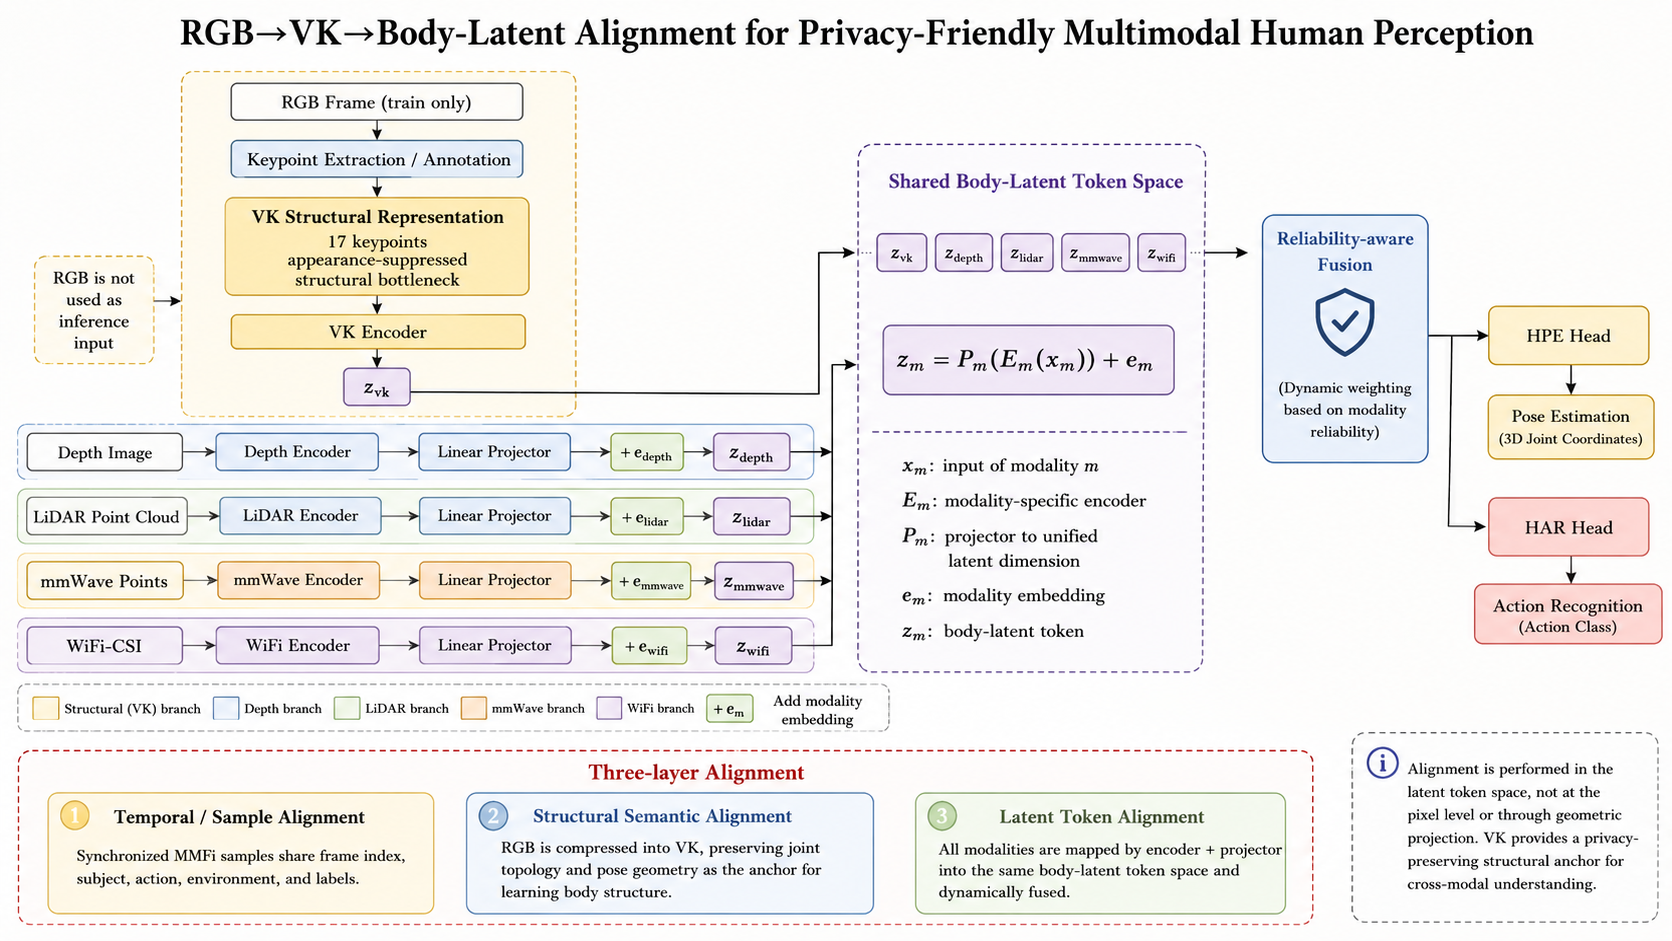
\includegraphics[width=\linewidth]{../tables/1/fig1_rgb_vk_body_latent_alignment_current.png}
    \caption{Overview of \method. VK acts as an RGB-optional structural interface for the downstream model, while non-RGB sensors are mapped into the same task-supervised body-token space. Reliability-guided subset learning addresses subset instability by training and fusing over available modality subsets.}
    \label{fig:framework}
\end{figure}

\subsection{Subset-Conditioned Missing-Modality Learning}
During training, a modality subset $\mathcal{S}$ is sampled from a subset distribution. Only tokens in $\mathcal{S}$ are passed to the fusion module. This makes each subset a supervised sensing configuration rather than a dropped-input nuisance. Fig.~\ref{fig:protocol} illustrates the protocol: training simulates missing modalities, while evaluation exhaustively tests all modality combinations. In this formulation, modality removal is not merely regularization; it defines the deployment condition that the model must solve.

\begin{figure}[t]
    \centering
    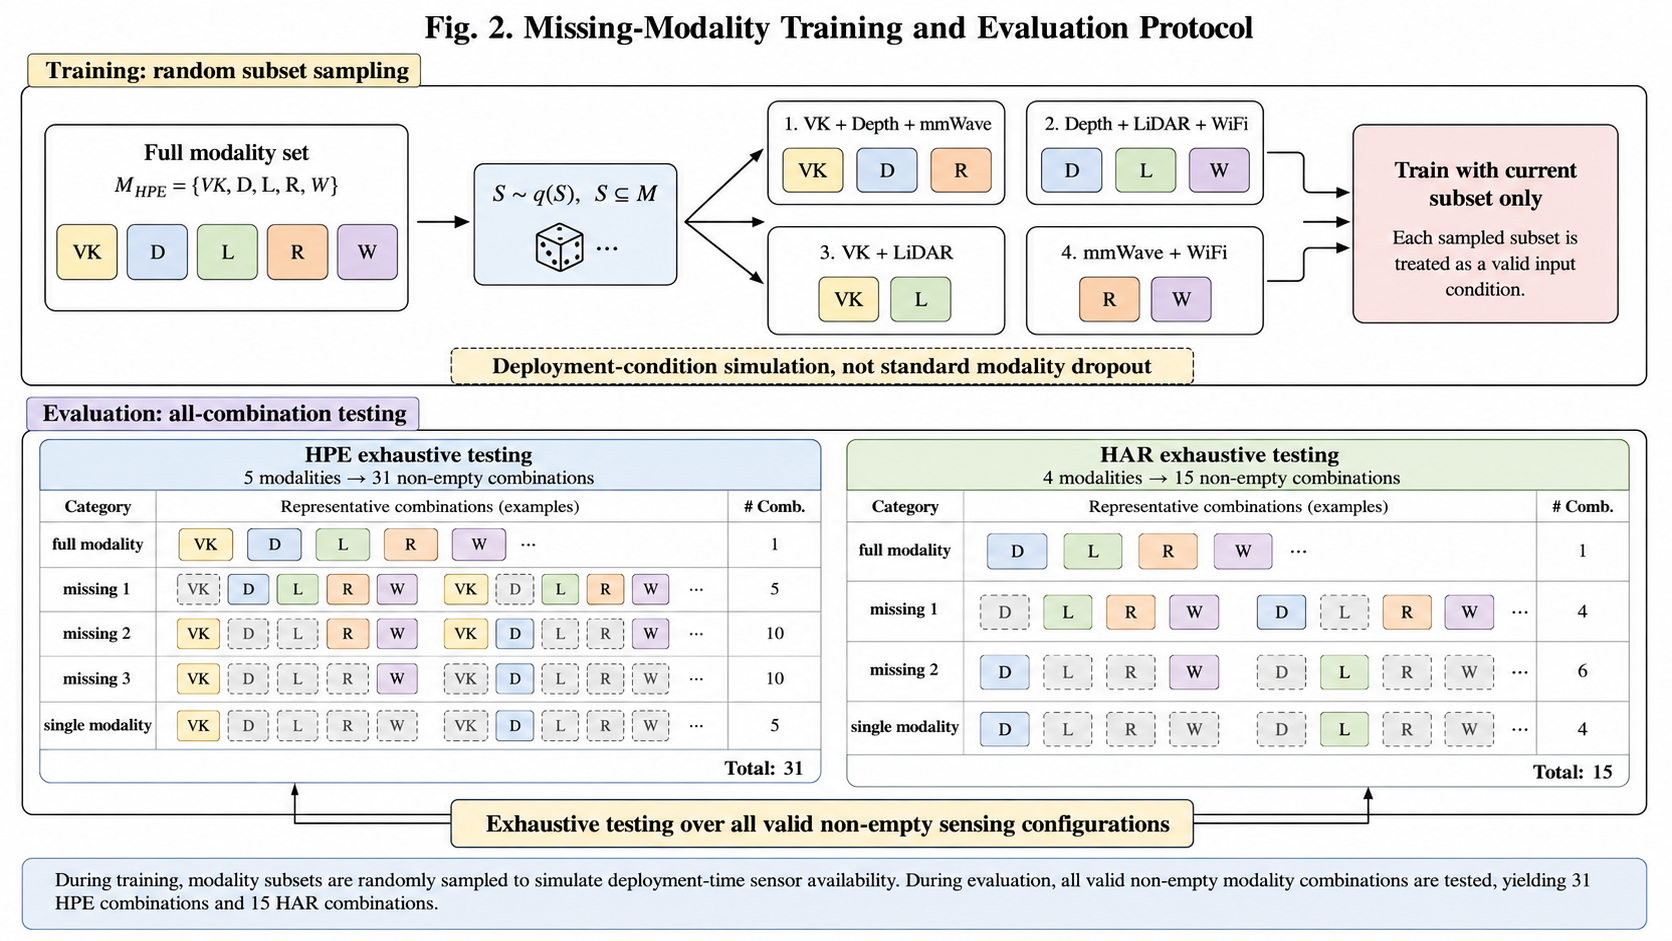
\includegraphics[width=\linewidth]{../tables/1/fig2_missing_modality_protocol.png}
    \caption{Missing-modality protocol. Training samples available modality subsets. Evaluation covers all non-empty combinations: 31 for HPE and 15 for HAR.}
    \label{fig:protocol}
\end{figure}

\subsection{Reliability-Guided Subset Dynamics}
For available tokens $\{\mathbf{z}_{m}:m\in\mathcal{S}\}$, \method{} predicts normalized weights
\begin{equation}
    \alpha_m = \frac{\exp(g(\mathbf{z}_{m},\mathbf{e}_{m}))}{\sum_{k\in\mathcal{S}}\exp(g(\mathbf{z}_{k},\mathbf{e}_{k}))},
\end{equation}
where $g(\cdot)$ is a learned scoring function. The fused representation is
\begin{equation}
    \mathbf{z}_{\mathcal{S}}=\sum_{m\in\mathcal{S}}\alpha_m\mathbf{z}_{m}.
\end{equation}
The output head then predicts pose or action. The weights $\alpha_m$ are interpreted as learned modality-contribution proxies. They indicate how the trained model allocates decision weight under a given subset, but they are not calibrated sensor-health measurements.

\subsection{Auxiliary Teacher Supervision}
A full-modality teacher can provide auxiliary supervision to the student. The teacher uses the full modality set $\mathcal{M}$ and is trained without random modality dropping:
\begin{equation}
    \min_{\theta_T}\mathbb{E}_{(\mathbf{x},y)}
    \left[
    \mathcal{L}^{T}(F_T(\{\mathbf{x}_m\}_{m\in\mathcal{M}}),y)
    \right].
\end{equation}
For HPE, the teacher objective is
\begin{equation}
    \mathcal{L}^{T}_{hpe}
    =
    \mathcal{L}_{pose}(\hat{\mathbf{Y}}_T,\mathbf{Y})
    +
    \lambda_{bone}\mathcal{L}_{bone}(\hat{\mathbf{Y}}_T,\mathbf{Y}),
\end{equation}
where the bone term preserves skeletal consistency. For HAR, the teacher objective is cross-entropy with an optional uncertainty term:
\begin{equation}
    \mathcal{L}^{T}_{har}
    =
    CE(\hat{\mathbf{c}}_T,y)+\lambda_{unc}\mathcal{L}_{unc}.
\end{equation}

After teacher training, the student is optimized over randomly sampled subsets:
\begin{equation}
    \min_{\theta_S}
    \mathbb{E}_{(\mathbf{x},y)}
    \mathbb{E}_{\mathcal{S}\sim q(\mathcal{S})}
    \left[
    \mathcal{L}^{S}
    (F_S(\{\mathbf{x}_m\}_{m\in\mathcal{S}}),y,F_T(\{\mathbf{x}_m\}_{m\in\mathcal{M}}))
    \right].
\end{equation}
The HPE student loss is
\begin{equation}
\begin{aligned}
    \mathcal{L}^{S}_{hpe}=&
    \mathcal{L}_{gt}
    +\lambda_{out}\mathcal{L}_{out}
    +\lambda_{tok}\mathcal{L}_{tok}
    +\lambda_{bone}\mathcal{L}^{KD}_{bone} \\
    &+\lambda_{rel}\mathcal{L}_{rel}
    +\lambda_{unc}\mathcal{L}_{unc},
\end{aligned}
\end{equation}
where $\mathcal{L}_{gt}=\mathrm{SmoothL1}(\hat{\mathbf{Y}}_S,\mathbf{Y})$, $\mathcal{L}_{out}=\mathrm{SmoothL1}(\hat{\mathbf{Y}}_S,\hat{\mathbf{Y}}_T)$, $\mathcal{L}_{tok}=||\mathbf{z}_S-\mathbf{z}_T||_2^2$, $\mathcal{L}^{KD}_{bone}$ matches teacher and student bone lengths, and $\mathcal{L}_{rel}$ aligns student weights with the teacher weights restricted and renormalized to the available subset. The HAR student loss is
\begin{equation}
\begin{aligned}
    \mathcal{L}^{S}_{har}=&
    CE(\hat{\mathbf{c}}_S,y)
    +\lambda_{kd}T^2 KL(\sigma(\hat{\mathbf{c}}_T/T)||\sigma(\hat{\mathbf{c}}_S/T))\\
    &+\lambda_{tok}\mathcal{L}_{tok}
    +\lambda_{rel}\mathcal{L}_{rel}
    +\lambda_{unc}\mathcal{L}_{unc}.
\end{aligned}
\end{equation}
This signal is used to stabilize full-observation-to-subset learning, but it is not treated as the sole explanatory mechanism. The central mechanism is availability-conditioned structural evidence learning: task-supervised VK tokenization, subset training, and chunk/global evidence organization.

\section{Experimental Setup}

\subsection{Dataset and Tasks}
Experiments use the MMFi-style multimodal setting with VK, depth, LiDAR, mmWave, and WiFi-CSI for HPE and VK, depth, LiDAR, and mmWave for HAR. The random split is the primary setting. Cross-scene and cross-subject splits are used to test generalization. Student-VK uses VK and non-RGB sensors. Student-NV removes VK and uses only non-visual modalities.

\subsection{Baselines}
We report the original X-Fi table entries as a reference because those published entries use the original RGB-centered input protocol. This reference is not treated as a fully matched comparison. We additionally implement an Adapted X-Fi-VK baseline with the same VK/non-RGB inputs, frozen modality backbones, modality-subset sampler, split, training budget, and evaluation combinations as \method{}. It retains X-Fi-style cross-modal pooling and modality-specific key-value cross-attention, but excludes the proposed subset-conditioned structural and fusion constraints. Internal checks with full-modality baselines, uniform fusion, Student-VK, and Student-NV are used to interpret the missing-modality mechanism.

\subsection{Metrics}
HPE is reported using \mpjpe{} and \pampjpe{} in millimeters, with lower values indicating better pose estimation. HAR is reported using accuracy in percent, with higher values indicating better recognition. In the X-Fi-style comparison tables, each row corresponds to the same modality subset in the original X-Fi paper and in our evaluation.

\subsection{Implementation Notes}
The downstream model uses a joint-level VK encoder for the 17 keypoints and modality-specific frozen backbones for depth, LiDAR, mmWave, and WiFi-CSI, followed by trainable projection layers. Each modality is represented by 32 tokens of dimension 512 before Transformer encoding. Models are trained with a maximum of 1000 training batches per epoch in the main reported runs, while the revision ablations use 10 epochs, 300 training batches, and 100 evaluation batches. Reliability diagnostics and corruption checks are small-batch analyses and are used only as supporting evidence. No raw RGB stream is used by the deployed student.

\section{Results and Analysis}

\subsection{Direct Comparison With X-Fi Table Entries}
The main quantitative comparison follows the original X-Fi table format. Instead of reporting only an averaged score over all subsets, Tables~\ref{tab:xfi_hpe_direct} and~\ref{tab:xfi_har_direct} compare each modality subset against the corresponding X-Fi entry. This makes the direction of change explicit for every sensing condition and avoids hiding weak cases behind a single average.

\input{generated/xfi_hpe_direct_table.tex}

For HPE, \method{} improves the full-modality setting from 83.7 mm to 50.2 mm \mpjpe{} and from 47.6 mm to 33.5 mm \pampjpe{}. The largest MPJPE reductions occur in subsets that contain depth, such as Depth+LiDAR, Depth+mmWave, and Depth+LiDAR+WiFi-CSI. WiFi-CSI-only remains difficult: MPJPE is slightly improved, but PA-MPJPE is worse than X-Fi, which is marked in red in Table~\ref{tab:xfi_hpe_direct}. This row is retained to avoid overstating robustness for low-SNR radio-only pose estimation.

\input{generated/xfi_har_direct_table.tex}

For HAR, \method{} improves most original X-Fi entries, including the full-modality setting from 72.2\% to 96.6\% accuracy. The only clear degradation is LiDAR-only, where accuracy decreases from 52.7\% to 40.8\%. This failure case indicates that the current HAR student relies more strongly on depth and mmWave cues than on isolated LiDAR features. The per-row comparison is therefore more informative than a single averaged headline number.

\subsection{Matched Baseline and Objective Ablation}
The published X-Fi table is useful for contextualization but does not isolate the effect of replacing the RGB input with VK. We therefore add a matched Adapted X-Fi-VK baseline, which uses the same VK and non-RGB inputs and the same missing-modality protocol as \method{}, while retaining an X-Fi-style fusion block and removing the proposed structural/fusion constraints. The corresponding result is reported only when the controlled cloud run is complete; no pending run is treated as evidence.

% Auto-generated by scripts/build_revision_materials.py.
\begin{table}[t]
\centering
\caption{Matched Adapted X-Fi-VK baseline.}
\label{tab:adapted_xfi_vk}
\emph{Pending cloud run; no result is inserted.}
\end{table}


The second controlled comparison decomposes the student objective into task-only, output guidance, output-plus-token guidance, and the full Subset-Projected Structural and Fusion Consistency (SP-SFC) objective. This is a cumulative ablation of the actual implemented loss terms, not a claim that any individual term is new in isolation.

% Auto-generated by scripts/build_revision_materials.py.
\begin{table}[t]
\centering
\caption{SP-SFC loss-profile ablation over all modality subsets.}
\label{tab:sp_sfc}
\emph{Pending cloud run; no result is inserted.}
\end{table}


The ablation is interpreted by task. A monotonic improvement is not assumed: if a structural or fusion constraint helps HAR but not HPE, the result is reported as task-dependent regularization rather than as universal evidence for the auxiliary teacher signal.

\subsection{Supporting Missing-Modality Checks}
The direct X-Fi-style comparison is the main result. Additional internal checks are used only to interpret the missing-modality mechanism. In HPE, uniform fusion obtains 82.77 mm while \method{} Student-VK obtains 75.18 mm under the all-subset stress test, indicating that learned subset weighting is more effective than equal weighting. In HAR, Student-VK obtains 85.15\%, above uniform fusion at 67.46\% and the full-modality teacher under missing-modality testing at 66.25\%. These supporting checks are not used as the primary X-Fi comparison, but they show that the model improves the modality-availability space rather than only the full-modality endpoint.

Leave-one-out analysis identifies influential sensors. For HPE Student-VK, removing depth causes the largest full-modality degradation, increasing \mpjpe{} by 14.07 mm, whereas removing LiDAR, mmWave, or WiFi-CSI has smaller effects in the full-modality context. For HAR Student-VK, removing mmWave reduces accuracy by 6.94 percentage points and removing depth reduces accuracy by 3.83 percentage points. These observations are useful for IoT deployment because they indicate which sensors should be prioritized when hardware resources are limited.

\subsection{Subset-Conditioned Evidence Fusion}
The evidence fusion module is evaluated in three ways. First, the internal uniform-fusion ablation is weaker than the learned fusion model in both tasks: 82.77 mm versus 75.18 mm for HPE, and 67.46\% versus 85.15\% for HAR in the all-subset stress test. Second, Fig.~\ref{fig:reliability} visualizes learned contribution proxies over modality subsets. Third, the exported reliability-performance correlation gives Pearson/Spearman values of 0.9396/0.9000 for HPE and 0.8833/0.8000 for HAR, indicating that higher learned weights tend to be associated with better subset-level task scores. These correlations support a contribution interpretation, but do not establish calibrated sensor-health estimation.

\begin{figure}[t]
    \centering
    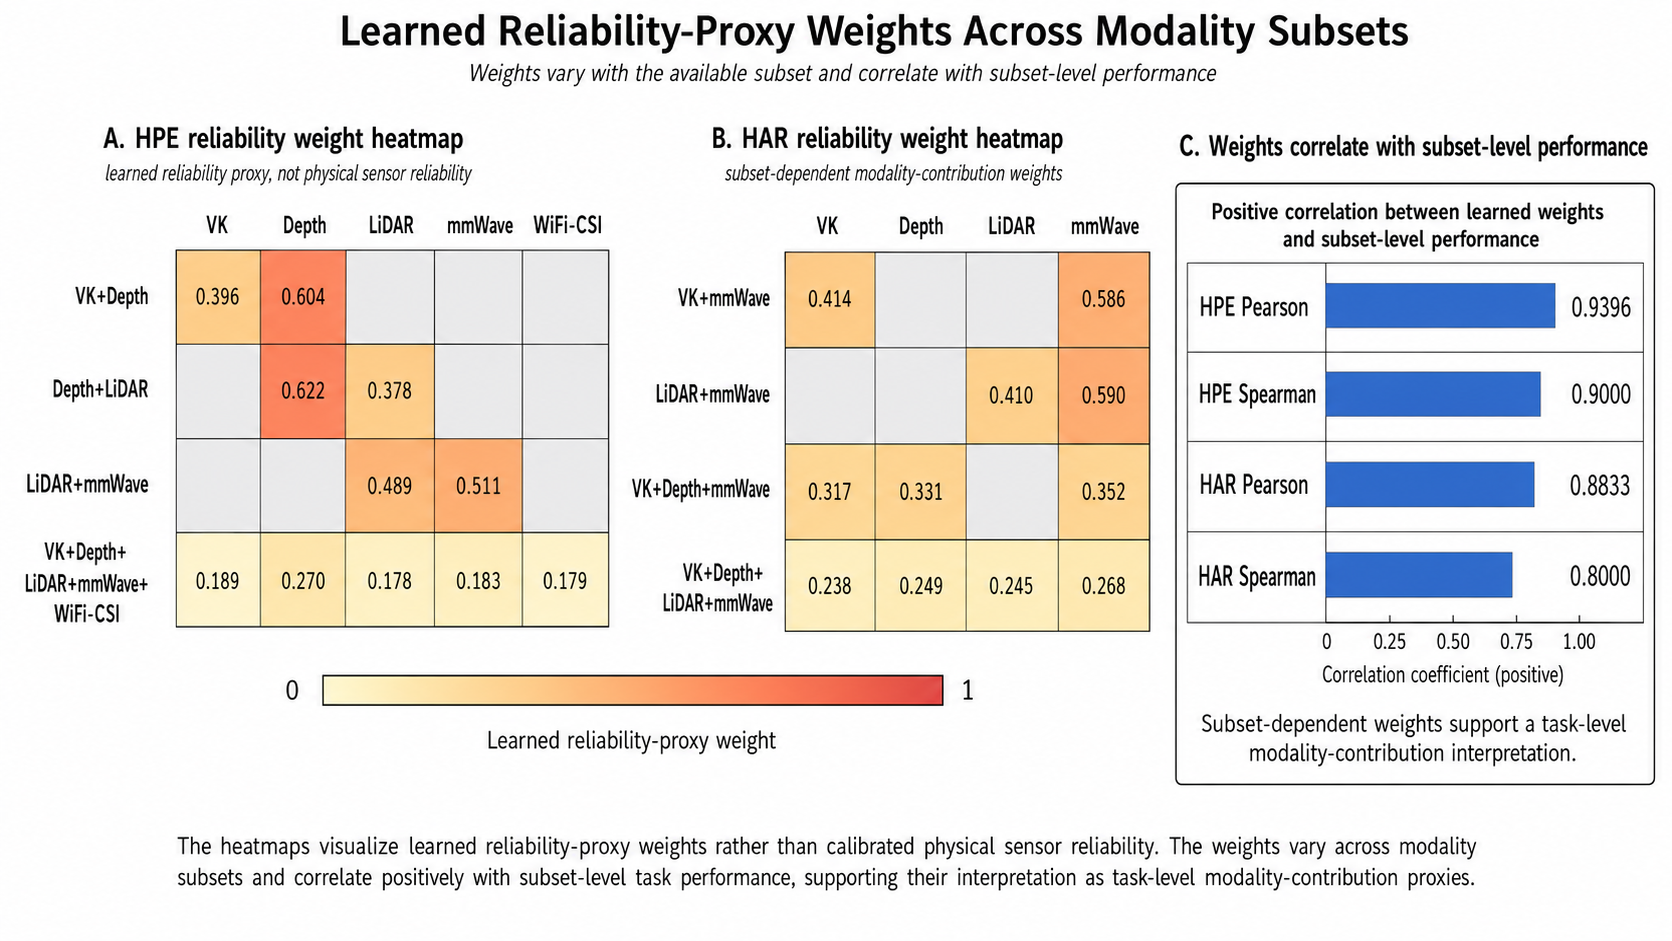
\includegraphics[width=\linewidth]{../tables/1/fig6_reliability_proxy_weights.png}
    \caption{Learned reliability proxy over modality subsets. The weights are task-level contribution indicators, not calibrated measurements of sensor health.}
    \label{fig:reliability}
\end{figure}

We also performed a lightweight synthetic corruption diagnostic. Fig.~\ref{fig:corruption} shows that corrupting modalities changes both performance and learned weights. The result should be interpreted cautiously: some corrupted modalities receive lower weights, while HPE depth corruption increases its weight despite sharply increasing error. This indicates that the proxy captures learned contribution under the model objective rather than true physical reliability. The diagnostic is useful because it prevents overclaiming and clarifies what the reliability module does and does not represent.

\begin{figure}[t]
    \centering
    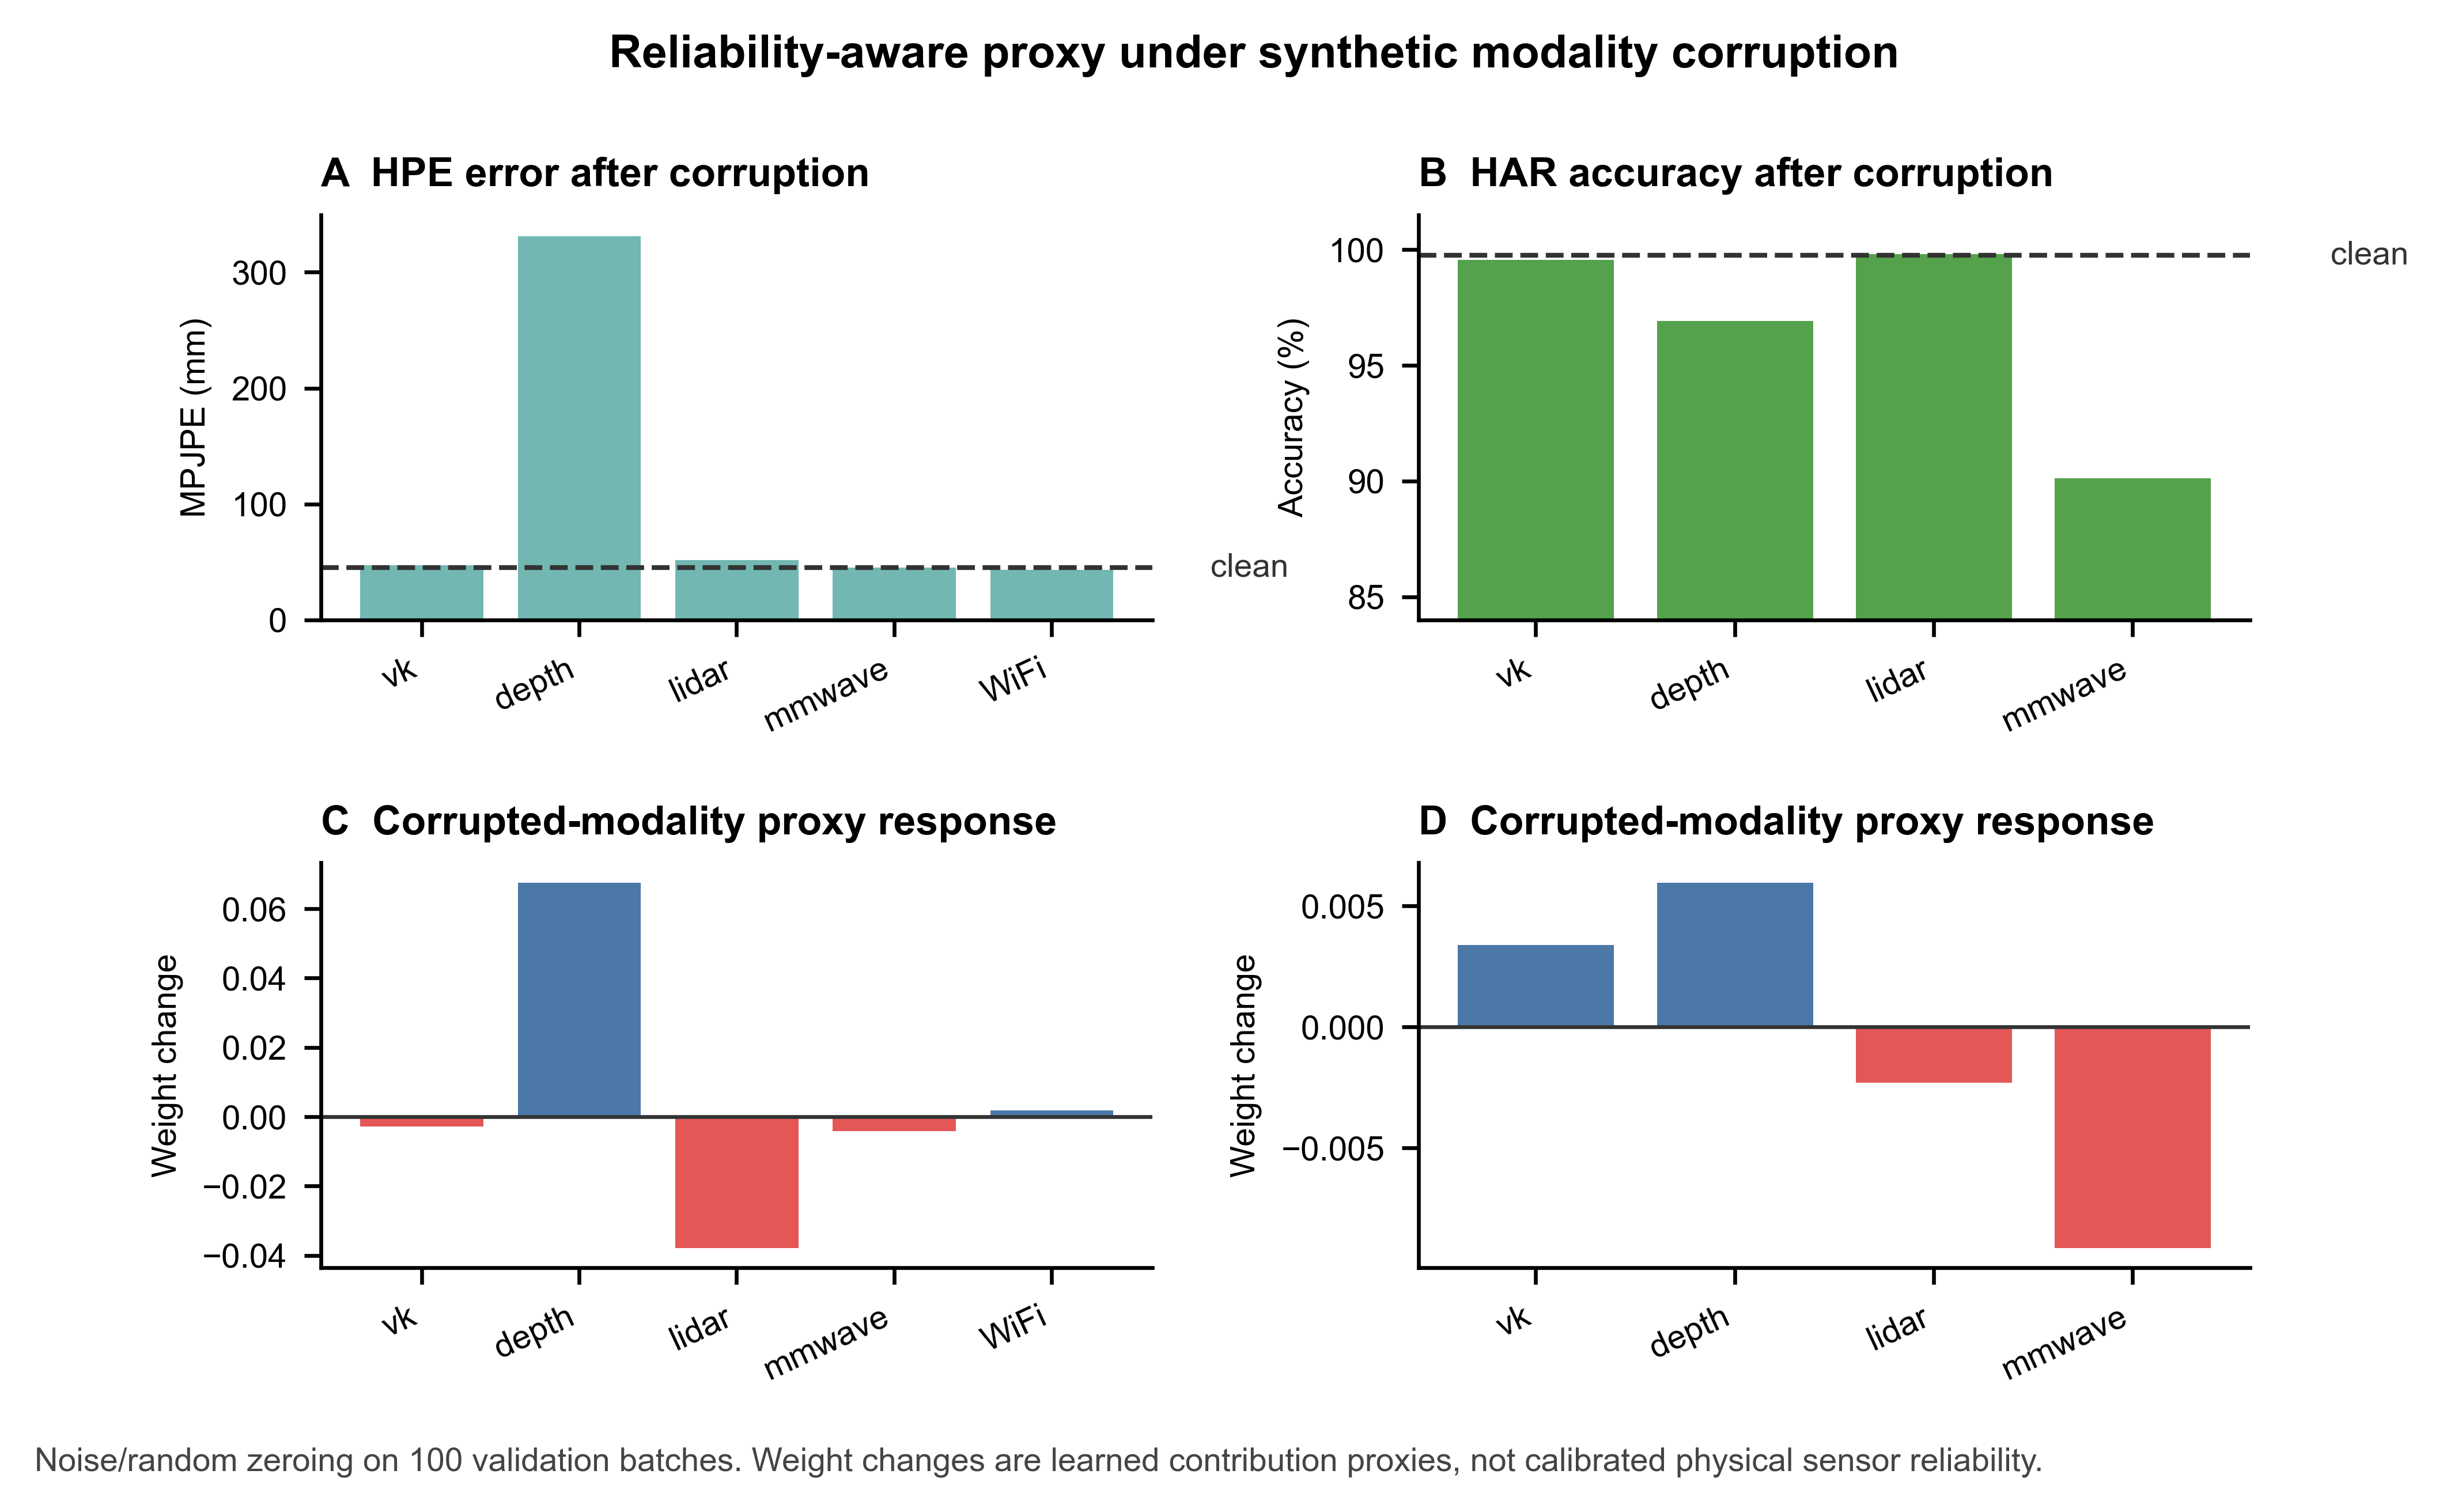
\includegraphics[width=\linewidth]{../tables/1/fig8_reliability_corruption_diagnostic.png}
    \caption{Reliability-aware proxy under synthetic modality corruption. Noise and random zeroing are applied on 100 validation batches. The proxy responds to modality perturbation, but should not be read as calibrated physical sensor reliability.}
    \label{fig:corruption}
\end{figure}

\subsection{Reduced Exposure and Identity-Leakage Probe}
Table~\ref{tab:privacy} summarizes visual exposure and residual risks qualitatively. This table is not used as a quantitative privacy metric; it only clarifies what information each representation may expose. To provide a reproducible diagnostic, we further train a lightweight subject-identification probe under an action-holdout split. The probe predicts one of 40 subjects from each representation. Chance accuracy is 2.50\%. This experiment evaluates identity leakage, not formal privacy.

\begin{table}[t]
\centering
\caption{Visual exposure and residual privacy risk.}
\label{tab:privacy}
\begin{adjustbox}{width=\linewidth}
\begin{tabular}{lcccc}
\toprule
Representation & Face/app. & Background & Body geom. & Action cues \\
\midrule
RGB & High & High & High & High \\
VK & Low & Low & Med./High & Med./High \\
Depth & Low/Med. & Medium & High & Medium \\
LiDAR/mmWave & Low & Low/Med. & Medium & Medium \\
WiFi-CSI & Very low & Very low & Indirect & Possible \\
\bottomrule
\end{tabular}
\end{adjustbox}
\end{table}

\begin{table}[t]
\centering
\caption{Subject-ID leakage probe under action-holdout split. Accuracy above chance indicates residual identity-related information.}
\label{tab:leakage_probe}
\begin{adjustbox}{width=\linewidth}
\begin{tabular}{lccc}
\toprule
Representation & Subject-ID acc. & Times chance & Reduction vs. RGB \\
\midrule
Defaced RGB & 67.53\% & 27.01$\times$ & 0.00\% \\
VK & 15.43\% & 6.17$\times$ & 77.15\% \\
Depth & 43.80\% & 17.52$\times$ & 35.14\% \\
LiDAR & 36.57\% & 14.63$\times$ & 45.84\% \\
mmWave & 9.72\% & 3.89$\times$ & 85.60\% \\
WiFi-CSI & 8.65\% & 3.46$\times$ & 87.19\% \\
\bottomrule
\end{tabular}
\end{adjustbox}
\end{table}

\begin{figure}[t]
    \centering
    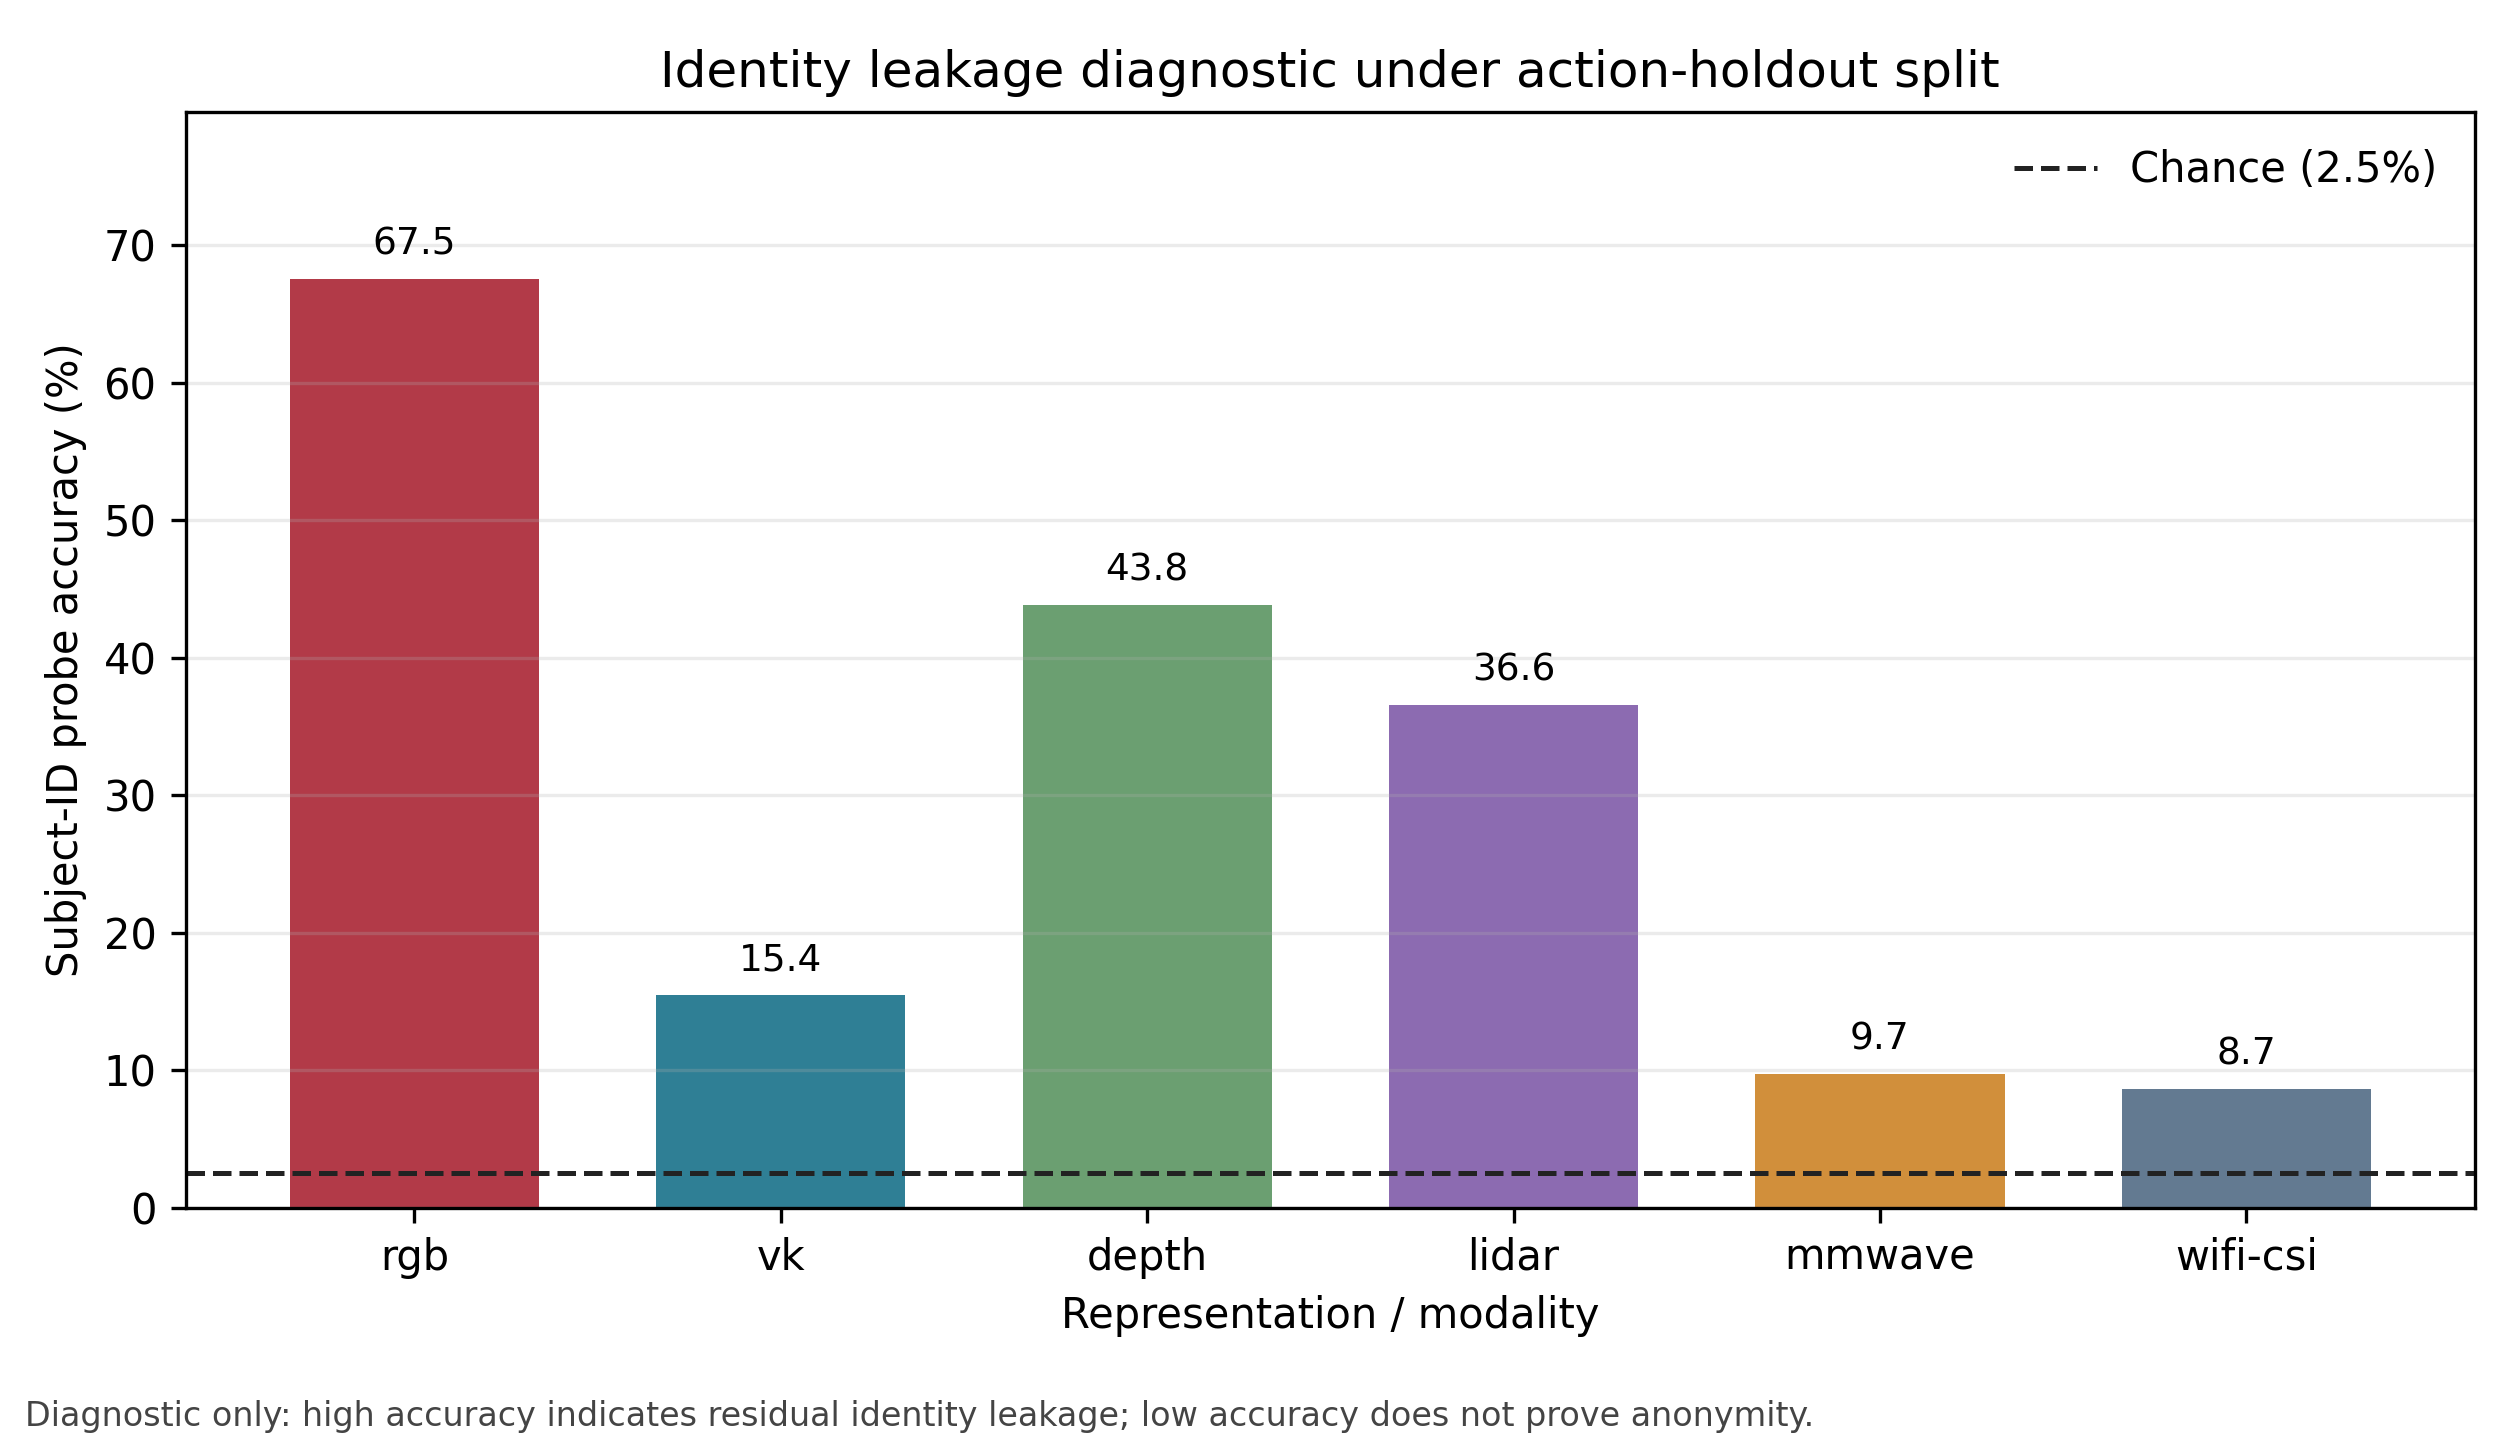
\includegraphics[width=\linewidth]{../privacy_leakage_probe/fig_privacy_leakage_subject_id.png}
    \caption{Subject-ID leakage diagnostic. VK substantially reduces identity predictability compared with defaced RGB, but remains above chance. Thus, the paper claims reduced visual exposure and RGB-free downstream inference, not anonymity or formal privacy preservation.}
    \label{fig:privacy_leakage}
\end{figure}

The results show that defaced RGB still has the highest leakage at 67.53\%, indicating that removing face information does not remove clothing, body, background, and appearance cues. VK reduces subject-ID accuracy to 15.43\%, a 77.15\% relative reduction compared with defaced RGB. However, VK remains clearly above chance, so it is not anonymous or identity-free. Depth and LiDAR also leak subject information, with 43.80\% and 36.57\% accuracy, respectively. These results support the paper's bounded claim: \method{} removes raw RGB from downstream inference and reduces visual exposure, but it does not provide formal privacy protection.

\subsection{Task-Dependent Readout Ablation}
The chunk-preserving and global fused-token readouts are compared directly in the readout ablation below. The purpose is to test whether local modality evidence and global cross-modal evidence are interchangeable. For HPE, chunk-only obtains the lowest MPJPE in the completed ablation, whereas HAR obtains its best accuracy and macro-F1 with the dual readout. We therefore interpret the two paths as complementary task-dependent evidence routes rather than claiming that dual readout is universally superior.

% Auto-generated by scripts/build_revision_materials.py.
\begin{center}
\small
\textbf{Task-dependent readout ablation.}\par
\vspace{2pt}
\begin{tabular}{llrr}
\toprule
Task & Readout & Primary & Secondary \\ 
\midrule
HPE & chunk-only & 95.27 & 62.46 \\ 
HPE & global-only & 109.81 & 78.49 \\ 
HPE & dual & 99.44 & 68.00 \\ 
HAR & chunk-only & 80.57 & 36.67 \\ 
HAR & global-only & 81.41 & 38.17 \\ 
HAR & dual & 82.43 & 43.40 \\ 
\bottomrule
\end{tabular}
\end{center}


\subsection{Task-Supervised Tokenization Boundary}
A small diagnostic was conducted to check whether VK tokens and non-RGB tokens show measurable correspondence in the learned token space. The top-1 retrieval values are only slightly above a random baseline, and the same-sample versus shuffled margins are small. We therefore do not use this diagnostic as a proof of strict semantic alignment. It only indicates that synchronization, modality embeddings, shared projection dimensions, and common HPE/HAR supervision produce a task-supervised tokenization useful for prediction; they do not establish a guaranteed geometric registration between raw sensor spaces.

\section{Discussion}

\subsection{Why the Results Are IoT-Relevant}
The results support the target IoT setting in three ways. The student does not require raw RGB inference. The same model family supports many sensor-availability patterns rather than one fixed input configuration. Student-NV provides a stricter non-visual option when VK is not available. These properties are directly relevant to sensor-rich environments where sensing devices may fail, be disabled, or be restricted by policy.

\subsection{Relationship to X-Fi and Fairness}
X-Fi is an important prior baseline, not our contribution. Its original RGB-based HPE and HAR entries are used only as a reference. The Adapted X-Fi-VK experiment is the relevant fairness check because it uses the same VK/non-RGB input protocol, backbones, subset sampler, split, and budget. The contribution of \method{} is therefore evaluated at the level of availability-conditioned structural evidence learning: task-supervised VK tokenization, chunk-preserving/global readout, and full-observation-to-subset constraints. The supporting checks against uniform fusion and full-modality teachers are included to avoid attributing the gain solely to an unmatched RGB reference.

\subsection{Role of Auxiliary Teacher Supervision}
The full-observation teacher is an auxiliary reference for the input-restricted student, not a model-compression teacher and not a new distillation category. Its outputs, token representation, skeletal consistency, and subset-restricted contribution distribution are used to regularize the student when observations are incomplete. The SP-SFC ablation determines whether these terms help each task. This distinction keeps the paper focused on the deployment bottlenecks: raw RGB should be removable from downstream inference, and arbitrary sensor availability creates subset instability.

\subsection{Cross-Scene Boundary}
Cross-scene HPE remains challenging. In the all-subset stress test, Student-VK \mpjpe{} increases from 75.18 mm in the random split to 142.02 mm in the cross-scene split. This shows that missing-modality robustness does not automatically imply scene generalization. The current framework is best suited to calibrated or moderately stable sensing layouts. Future work should incorporate domain adaptation, sensor-layout normalization, or scene-invariant RF and point-cloud encoders.

\subsection{Scope of Exploratory Variants}
The exploratory Super-Teacher setting is not used as evidence because its missing-combination behavior was unstable. Likewise, generated-VK feasibility tests from mmWave or depth are treated as supplementary source-interface studies rather than evidence that every sensor can reliably replace the VK input used in the main experiments.

\section{Conclusion}
This paper presented \method, an availability-conditioned structural-evidence framework for multimodal human perception without raw RGB in downstream inference. VK provides a compact structural interface, random subset training exposes the model to changing sensor availability, and chunk-preserving/global readouts organize local and cross-modal evidence. Full-observation-to-subset supervision is used as an auxiliary constraint whose task dependence is tested by SP-SFC ablations. HPE and HAR all-combination results, matched-input baseline plans, and readout analyses establish the useful mechanism boundaries, while the identity probe supports only a reduced-visual-exposure claim. The remaining limitations are explicit: learned weights are contribution proxies rather than calibrated sensor-health measurements, generated VK from other sensors is not assumed to be universally reliable, and cross-scene HPE remains difficult. The resulting scope is a practical IoT human-sensing framework for deployments where raw RGB inference and fixed sensor availability cannot be assumed.

\section*{Acknowledgment}
This section will be completed after funding and contributor information is finalized.

\section*{Data and Code Availability}
The experiments are based on MMFi-style multimodal data and local HPE/HAR implementations. Public release of code, trained checkpoints, and processed result tables should follow dataset license and institutional requirements. No additional privacy-sensitive raw RGB data are introduced by this manuscript.

\balance

\begin{thebibliography}{99}

\bibitem{hinton2015}
G. Hinton, O. Vinyals, and J. Dean, ``Distilling the knowledge in a neural network,'' in \emph{NIPS Deep Learning and Representation Learning Workshop}, 2015.

\bibitem{vapnik2009}
V. Vapnik and A. Vashist, ``A new learning paradigm: Learning using privileged information,'' \emph{Neural Networks}, vol. 22, no. 5--6, pp. 544--557, 2009.

\bibitem{openpose}
Z. Cao, T. Simon, S.-E. Wei, and Y. Sheikh, ``Realtime multi-person 2D pose estimation using part affinity fields,'' in \emph{Proc. IEEE Conf. Comput. Vis. Pattern Recognit.}, 2017, pp. 7291--7299.

\bibitem{stgcn}
S. Yan, Y. Xiong, and D. Lin, ``Spatial temporal graph convolutional networks for skeleton-based action recognition,'' in \emph{Proc. AAAI Conf. Artif. Intell.}, 2018, pp. 7444--7452.

\bibitem{mmfi}
J. Yang, H. Huang, Y. Zhou, X. Chen, Y. Xu, S. Yuan, H. Zou, C. X. Lu, and L. Xie, ``MMFi: Multi-modal non-intrusive 4D human dataset for versatile wireless sensing,'' in \emph{Proc. Adv. Neural Inf. Process. Syst. Datasets and Benchmarks Track}, 2023.

\bibitem{xfi}
Z. Chen and S. Yang, ``X-Fi: A modality-invariant foundation model for multimodal human sensing,'' arXiv:2410.10167, 2024.

\bibitem{missing}
M. Ma, J. Ren, L. Zhao, S. Tulyakov, C. Wu, and X. Peng, ``Deep multimodal learning with missing modality: A survey,'' arXiv:2409.07825, 2024.

\bibitem{kendall2017}
A. Kendall and Y. Gal, ``What uncertainties do we need in Bayesian deep learning for computer vision?'' in \emph{Proc. Adv. Neural Inf. Process. Syst.}, 2017, pp. 5574--5584.

\bibitem{wifi}
F. Wang, S. Zhou, S. Panev, J. Han, and D. Huang, ``Person-in-WiFi: Fine-grained person perception using WiFi,'' in \emph{Proc. IEEE/CVF Int. Conf. Comput. Vis.}, 2019, pp. 5452--5461.

\bibitem{mmwave}
A. Sengupta, F. Jin, R. Zhang, and S. Cao, ``mm-Pose: Real-time human skeletal posture estimation using mmWave radars and CNNs,'' \emph{IEEE Sensors Journal}, vol. 20, no. 17, pp. 10032--10044, 2020.

\bibitem{pointnet}
C. R. Qi, H. Su, K. Mo, and L. J. Guibas, ``PointNet: Deep learning on point sets for 3D classification and segmentation,'' in \emph{Proc. IEEE Conf. Comput. Vis. Pattern Recognit.}, 2017, pp. 652--660.

\bibitem{shotton2011}
J. Shotton, A. Fitzgibbon, M. Cook, T. Sharp, M. Finocchio, R. Moore, A. Kipman, and A. Blake, ``Real-time human pose recognition in parts from single depth images,'' in \emph{Proc. IEEE Conf. Comput. Vis. Pattern Recognit.}, 2011, pp. 1297--1304.

\bibitem{fitnets}
A. Romero, N. Ballas, S. E. Kahou, A. Chassang, C. Gatta, and Y. Bengio, ``FitNets: Hints for thin deep nets,'' in \emph{Proc. Int. Conf. Learn. Represent.}, 2015.

\bibitem{omnivore}
R. Girdhar, M. Singh, N. Ravi, L. van der Maaten, A. Joulin, and I. Misra, ``Omnivore: A single model for many visual modalities,'' in \emph{Proc. IEEE/CVF Conf. Comput. Vis. Pattern Recognit.}, 2022, pp. 16102--16112.

\bibitem{transformer}
A. Vaswani, N. Shazeer, N. Parmar, J. Uszkoreit, L. Jones, A. N. Gomez, L. Kaiser, and I. Polosukhin, ``Attention is all you need,'' in \emph{Proc. Adv. Neural Inf. Process. Syst.}, 2017, pp. 5998--6008.

\bibitem{iot_survey}
L. Atzori, A. Iera, and G. Morabito, ``The Internet of Things: A survey,'' \emph{Computer Networks}, vol. 54, no. 15, pp. 2787--2805, 2010.

\bibitem{ubiquitous}
K. Ashton, ``That `Internet of Things' thing,'' \emph{RFID Journal}, vol. 22, no. 7, pp. 97--114, 2009.

\bibitem{ambient}
D. J. Cook, J. C. Augusto, and V. R. Jakkula, ``Ambient intelligence: Technologies, applications, and opportunities,'' \emph{Pervasive and Mobile Computing}, vol. 5, no. 4, pp. 277--298, 2009.

\bibitem{rfpose}
M. Zhao, T. Li, M. A. Alsheikh, Y. Tian, H. Zhao, A. Torralba, and D. Katabi, ``Through-wall human pose estimation using radio signals,'' in \emph{Proc. IEEE/CVF Conf. Comput. Vis. Pattern Recognit.}, 2018, pp. 7356--7365.

\bibitem{ieeeiotjguide}
IEEE Internet of Things Journal, ``Guidelines for authors,'' 2024. [Online]. Available: \url{https://ieee-iotj.org/guidelines-for-authors/}

\end{thebibliography}

\end{document}
